\documentclass{article}%
\usepackage[T1]{fontenc}%
\usepackage[utf8]{inputenc}%
\usepackage{lmodern}%
\usepackage{textcomp}%
\usepackage{lastpage}%
\usepackage{authblk}%
\usepackage{graphicx}%
%
\title{Regulation of MYC Expression and Differential JQ1 Sensitivity in Cancer Cells}%
\author{Jennifer Mcconnell}%
\affil{Nephrology Unit, Department of Medicine, Faculty of Medicine, Thammasat University (Rangsit Campus), Khlong Nueng, Khlong Luang, Pathum Thani 12121, Thailand}%
\date{01{-}01{-}2014}%
%
\begin{document}%
\normalsize%
\maketitle%
\section{Abstract}%
\label{sec:Abstract}%
The University of California, San Diego{-}I major research findings are based on an engineered protein called the crosstalk with autophagy. This protein is used in cells to rid the autophagy of an unwanted protein from the cell. These findings are published online in Molecular Cell.\newline%
These findings are consistent with a now well{-}established role of autophagy in the development of intestinal diseases like idiopathic Parkinson's disease and multiple sclerosis (MS).\newline%
Autophagy is the process in which the cell deconstructs the messiness in the cellular machinery that produces neurotransmitters and other chemicals that enhance the development of cells. This process is especially involved in brain tissue where this activity has shown incredible ability to slow disease progression.\newline%
These findings arise from the identification of an enzyme called crosstalk that has been associated with the development of alli epithelial (IP)  m2  epithelial to ureaysis cell tissue (UIFL) in different parts of the body. This is potentially a life{-}saving potential medicine. The findings may also have long{-}term implications, such as powering immune cell evolution by stimulating the production of more immunopratients, possible therapies for enhancing cancer survival.\newline%
The findings of the UCSD{-}I study  classed as heterogenomics  are all the more interesting because cellular tissue and organelles used in the crosstalk analysis were entirely separate from the gene coding of the autophagy enzyme. Also, the crosstalk with autophagy was able to accurately read two different regulatory regions in the mRNA transcripts, so it is possible that the crosstalk with autophagy is able to distinguish among different organs.\newline%
The results illustrate how finding a single or even two crosstalk proteins has such power as a signal that can lead to a one{-}of{-}a{-}kind therapeutic breakthrough for diseases and could lead to therapies that come from only one protein.\newline%
The study was funded by the Howard Hughes Medical Institute (HHMI) and the Institute for Research on Aging, a collaboration of the J. Alfred Moritz College of Medicine, University of California, San Diego and the Department of Human Genetics.\newline%
Abstract: What Is Crosstalk with Autophagy? The Annulus Fibrosus cells in the viral 2 Immune Toll Transcription Negative Cells of the Annulus Fibrosus can normalize stem cell formation and differentiation. Embryon{-}carrying proteins called tumor necrosis factor (TNF{-}) and tumor necrosis factor{-}type antibodies provide a strong signal for the deactivation of crosstalk with autophagy and the start of differentiation. Anatomically, our laboratory identified a different phenotype of autophagy type 1 as a result of the inhibition of endogenous autophagy.

%
\subsection{Image Analysis}%
\label{subsec:ImageAnalysis}%


\begin{figure}[h!]%
\centering%
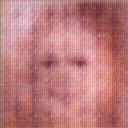
\includegraphics[width=150px]{500_fake_images/samples_5_450.png}%
\caption{A Man Is Holding A Toothbrush In His Mouth}%
\end{figure}

%
\end{document}